\documentclass[12pt,a4paper]{article}
\usepackage[utf8]{inputenc}
\usepackage[margin=2.5cm]{geometry}
\usepackage{graphicx}
\usepackage{float}
\usepackage{listings}
\usepackage{xcolor}
\usepackage{hyperref}
\usepackage{tikz}
\usetikzlibrary{positioning, arrows.meta, shapes.geometric}
\usepackage{booktabs}
\usepackage{longtable}
\usepackage{enumitem}
\usepackage{amsmath}
\usepackage{amssymb}
\usepackage{fancyhdr}
\usepackage{tocloft}
\usepackage{titlesec}
\usepackage{verbatim}

% Code listing style
\definecolor{codebg}{RGB}{245,245,245}
\definecolor{codegreen}{RGB}{0,128,0}
\definecolor{codegray}{RGB}{128,128,128}
\definecolor{codepurple}{RGB}{128,0,128}
\definecolor{codeblue}{RGB}{0,0,180}

\lstdefinestyle{pythonstyle}{
    backgroundcolor=\color{codebg},
    basicstyle=\ttfamily\small,
    breaklines=true,
    captionpos=b,
    commentstyle=\color{codegreen},
    keywordstyle=\color{codeblue}\bfseries,
    stringstyle=\color{codepurple},
    numberstyle=\tiny\color{codegray},
    numbers=left,
    numbersep=5pt,
    frame=single,
    rulecolor=\color{black!30},
    showstringspaces=false,
    tabsize=4,
    language=Python
}

\lstdefinestyle{textstyle}{
    backgroundcolor=\color{codebg},
    basicstyle=\ttfamily\small,
    breaklines=true,
    frame=single,
    rulecolor=\color{black!30},
    showstringspaces=false,
}

\lstset{style=pythonstyle}

% Header/Footer
\pagestyle{fancy}
\fancyhf{}
\rhead{SDN Controller Project}
\lhead{\leftmark}
\rfoot{Page \thepage}

% Title formatting
\titleformat{\section}{\Large\bfseries}{}{0em}{}[\titlerule]
\titleformat{\subsection}{\large\bfseries}{}{0em}{}

\hypersetup{
    colorlinks=true,
    linkcolor=blue!70!black,
    urlcolor=blue!70!black,
    citecolor=blue!70!black
}



% ============================================================
% TITLE PAGE
% ============================================================
% 1. ?????????????????????????
\begin{document}
\begin{center}
{\Large\bfseries SDN Controller Project Documentation}

\vspace{0.2cm}
\end{center}


% % ============================================================
% % TABLE OF CONTENTS
% % ============================================================
% \tableofcontents
% \newpage

% ============================================================
% 1. OVERALL ARCHITECTURE
% ============================================================
\section{Overall Architecture}

This project implements a fully-featured Software-Defined Networking (SDN) controller built upon the \textbf{os-ken} framework (the community-maintained successor to Ryu) and the \textbf{OpenFlow 1.0} protocol. The controller serves as the centralised intelligence of the network, making all forwarding, addressing, naming, translation, and security decisions on behalf of the data-plane switches.

The system follows the canonical three-tier SDN architecture:

\begin{figure}[H]
\centering
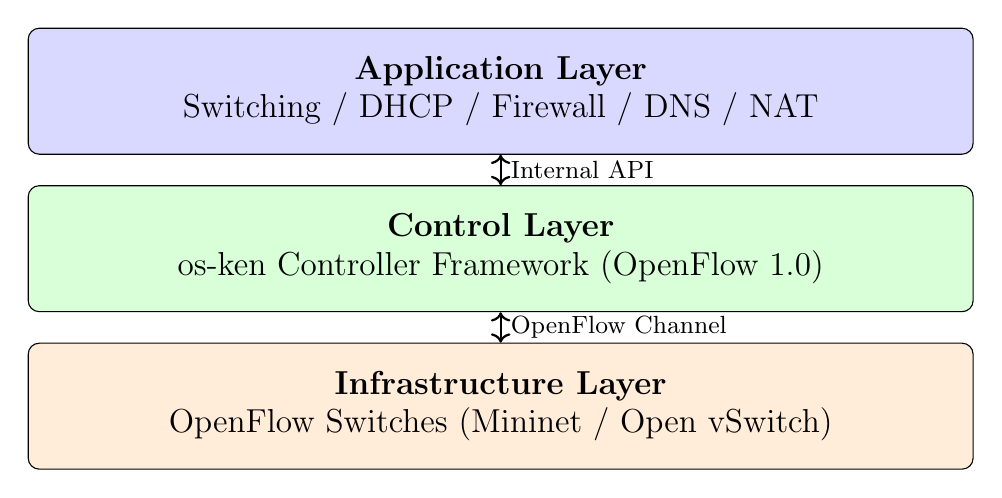
\begin{tikzpicture}[
    layer/.style={draw, rounded corners, minimum width=12cm, minimum height=1.6cm, align=center, font=\large},
    arr/.style={-{Stealth[length=3mm]}, thick}
]
\node[layer, fill=blue!15] (app) at (0, 4) {\textbf{Application Layer}\\Switching / DHCP / Firewall / DNS / NAT};
\node[layer, fill=green!15] (ctrl) at (0, 2) {\textbf{Control Layer}\\os-ken Controller Framework (OpenFlow 1.0)};
\node[layer, fill=orange!15] (infra) at (0, 0) {\textbf{Infrastructure Layer}\\OpenFlow Switches (Mininet / Open vSwitch)};

\draw[arr, <->] (app.south) -- (ctrl.north) node[midway, right, font=\small] {Internal API};
\draw[arr, <->] (ctrl.south) -- (infra.north) node[midway, right, font=\small] {OpenFlow Channel};
\end{tikzpicture}
\caption{Three-tier SDN Architecture}
\end{figure}

The \textbf{Infrastructure Layer} consists of OpenFlow-enabled switches (realised via Open vSwitch within Mininet) that forward packets strictly according to their flow tables. These switches have no autonomous forwarding logic; they rely entirely on the controller for decision-making.

The \textbf{Control Layer} is the os-ken framework itself, which manages the OpenFlow connections to each switch, dispatches events (such as PacketIn, topology changes, and port status updates), and provides the programming interface for flow table manipulation.

The \textbf{Application Layer} hosts five cooperating modules that together implement the full network functionality. When a switch encounters a packet that matches no flow entry, it forwards the packet to the controller via a \texttt{PacketIn} message. The controller's packet processing pipeline inspects the packet, determines the appropriate action (DHCP reply, ARP proxy response, DNS answer, NAT rewriting, or shortest-path forwarding), and either sends a direct \texttt{PacketOut} reply or installs proactive flow entries via \texttt{FlowMod} messages so that subsequent packets of the same flow are handled entirely in the data plane without controller involvement.

% ============================================================
% 2. PROJECT OVERVIEW
% ============================================================
\section{Project Overview}

This project delivers a comprehensive SDN solution that goes beyond basic L2 switching to provide a complete network services stack. The five major functionalities are summarised below:

\begin{table}[H]
\centering
\begin{tabular}{@{}lp{9cm}@{}}
\toprule
\textbf{Module} & \textbf{Description} \\
\midrule
Shortest-Path Switching & Discovers the network topology via LLDP-based link detection, computes shortest paths using graph algorithms (Dijkstra, Bellman-Ford, Floyd-Warshall), and installs forwarding flow entries along the computed paths. Supports link failover and automatic path recomputation. \\
\addlinespace
DHCP & Allocates IP addresses from a configurable pool (192.168.1.2--192.168.1.100), handling the full DISCOVER/OFFER/REQUEST/ACK lifecycle with lease management, duplicate prevention, and stale offer expiration. \\
\addlinespace
Firewall & Loads deny rules from an external JSON configuration file, normalises CIDR notation and protocol identifiers, and installs high-priority drop flows (priority 60000) to block matching traffic before it reaches forwarding rules. \\
\addlinespace
DNS & Provides lightweight name resolution within the SDN, automatically registering host names upon discovery and responding to A and PTR queries via raw PacketOut. \\
\addlinespace
NAT & Performs SNAT/DNAT between internal (10.0.1.0/24) and external (10.0.2.0/24) subnets, with full connection tracking, ephemeral port allocation, and header rewriting for ICMP, TCP, and UDP. \\
\bottomrule
\end{tabular}
\caption{Module Summary}
\end{table}

The controller is designed to be modular: each service (DHCP, DNS, Firewall, NAT) is implemented in its own Python module and integrated into the main controller's \texttt{PacketIn} pipeline. This separation of concerns allows individual modules to be developed, tested, and debugged independently while still cooperating seamlessly at runtime.

% ============================================================
% 3. STRUCTURE OVERVIEW
% ============================================================
\section{Structure Overview}

\subsection{Packet Processing Pipeline}

When a packet arrives at the controller, it traverses a carefully ordered processing pipeline. Each stage inspects the packet and either handles it (returning early) or passes it to the next stage. This design ensures that higher-priority services (such as DHCP and ARP) are processed first, while general forwarding acts as the final catch-all.

\begin{figure}[H]
\centering
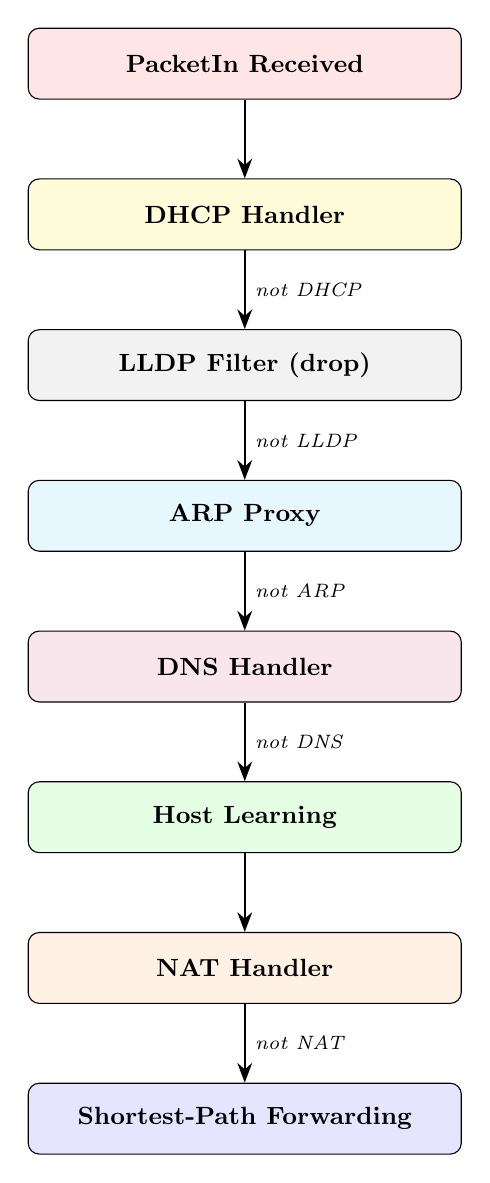
\begin{tikzpicture}[
    node distance=1.0cm,
    block/.style={draw, rounded corners, minimum width=5.5cm, minimum height=0.9cm, align=center, font=\small\bfseries},
    arr/.style={-{Stealth[length=2.5mm]}, thick}
]
\node[block, fill=red!10] (a) {PacketIn Received};
\node[block, fill=yellow!15, below=of a] (b) {DHCP Handler};
\node[block, fill=gray!10, below=of b] (b2) {LLDP Filter (drop)};
\node[block, fill=cyan!10, below=of b2] (c) {ARP Proxy};
\node[block, fill=purple!10, below=of c] (d) {DNS Handler};
\node[block, fill=green!10, below=of d] (e) {Host Learning};
\node[block, fill=orange!10, below=of e] (f) {NAT Handler};
\node[block, fill=blue!10, below=of f] (g) {Shortest-Path Forwarding};

\draw[arr] (a) -- (b);
\draw[arr] (b) -- (b2) node[midway, right, font=\scriptsize\itshape] {not DHCP};
\draw[arr] (b2) -- (c) node[midway, right, font=\scriptsize\itshape] {not LLDP};
\draw[arr] (c) -- (d) node[midway, right, font=\scriptsize\itshape] {not ARP};
\draw[arr] (d) -- (e) node[midway, right, font=\scriptsize\itshape] {not DNS};
\draw[arr] (e) -- (f);
\draw[arr] (f) -- (g) node[midway, right, font=\scriptsize\itshape] {not NAT};
\end{tikzpicture}
\caption{Packet Processing Pipeline --- each stage returns early when it handles the packet}
\end{figure}

\subsection{Module Responsibilities}

The controller consists of five cooperating modules, each with clearly defined responsibilities:

\begin{itemize}[leftmargin=1.5cm]
    \item \textbf{ControllerApp} (\texttt{controller.py}) --- The main application class that handles topology events (switch join/leave, link add/delete, port modifications), the \texttt{PacketIn} processing pipeline, host learning, ARP proxy, shortest-path computation, and flow table management. It orchestrates the other modules by invoking them at appropriate points in the pipeline.
    \item \textbf{DHCPServer} (\texttt{dhcp.py}) --- Implements a complete DHCP server that allocates IP addresses from a configurable pool, manages lease lifetimes, handles the four-message handshake (DISCOVER/OFFER/REQUEST/ACK), and releases addresses upon client departure or lease expiration.
    \item \textbf{Firewall} (\texttt{firewall.py}) --- Loads security policy rules from an external JSON file, normalises CIDR addresses and protocol identifiers, and proactively installs high-priority drop flows on every switch to block prohibited traffic before it is ever forwarded.
    \item \textbf{DNSServer} (\texttt{dns\_server.py}) --- Provides in-controller DNS resolution for learned hosts. It maintains bidirectional hostname-to-IP mappings, answers A record and PTR record queries, and returns appropriate error codes (NXDOMAIN, SERVFAIL) for unknown or unsupported queries.
    \item \textbf{NAT} (\texttt{nat.py}) --- Performs Network Address Translation between internal and external subnets. It rewrites IP and transport headers, manages a connection tracking table with ephemeral port allocation, and handles both SNAT (outbound) and DNAT (inbound) directions for ICMP, TCP, and UDP.
\end{itemize}

\subsection{Project File Tree}

\begin{lstlisting}[style=textstyle]
project/
|-- controller.py            # Controller app: topology + shortest-path forwarding
|-- dhcp.py                  # DHCP server
|-- firewall.py              # Firewall rule loading and installation
|-- dns_server.py            # DNS server (A and PTR records)
|-- nat.py                   # NAT module (SNAT/DNAT)
|-- ofctl_utilis.py          # OpenFlow utility library
|-- tests/
|   |-- switching_test/
|   |   +-- test_network.py  # Switching test script
|   |-- dhcp_test/
|   |   |-- test_network.py         # DHCP interactive test (basic, release, duplicate)
|   |   |-- test_network_overflow.py # DHCP overflow test (more hosts than IPs)
|   |   +-- test_lease_expiry.py    # DHCP lease expiration test (timed expiry)
|   |-- firewall_test/
|   |   +-- test_network.py  # Firewall test script
|   |-- dns_test/
|   |   |-- test_network_dns.py  # DNS interactive test
|   |   +-- ci/
|   |       +-- test_dns.py      # DNS CI test
|   +-- nat_test/
|       |-- test_network_nat.py  # NAT interactive test
|       +-- ci/
|           +-- test_nat.py      # NAT CI test
|-- docs/
|   |-- controller_zh.md
|   |-- dhcp.md
|   |-- firewall.md
|   |-- dns.md
|   +-- nat.md
|-- README.md
+-- requirements.txt
\end{lstlisting}

% ============================================================
% 4. CONTROLLER
% ============================================================
\section{Controller --- Shortest-Path Switching}

\subsection{Functionality}

The \texttt{ControllerApp} class is the central component of the entire SDN system. It is responsible for maintaining an accurate real-time view of the network topology and computing optimal forwarding paths between all pairs of communicating hosts. Its major responsibilities include:

\begin{itemize}[leftmargin=1.5cm]
    \item \textbf{Topology Discovery and Maintenance:} The controller listens for OpenFlow events including switch feature replies (new switch registration), link addition/deletion notifications, and port status changes. These events are used to build and maintain an adjacency graph of the network in real time.
    \item \textbf{Host Learning:} When a host first sends traffic (or is detected via topology events), the controller records its MAC address, IP address, the switch it is connected to, and the port number. This information is essential for computing end-to-end paths.
    \item \textbf{ARP Proxy:} Rather than flooding ARP requests across the entire network, the controller intercepts ARP queries and responds directly from its ARP table when the target is known. This eliminates broadcast storms and reduces unnecessary traffic. The ARP proxy also handles special addresses such as the DNS server IP (192.168.1.1) and the NAT external IP (10.0.2.100).
    \item \textbf{Shortest-Path Routing:} The controller implements three classical shortest-path algorithms---Dijkstra, Bellman-Ford, and Floyd-Warshall---providing flexibility and redundancy in path computation. All link weights are treated as unity (hop count metric).
    \item \textbf{Flow Installation:} Once a shortest path is determined, the controller installs flow entries on every switch along the path so that subsequent packets of the same flow are forwarded entirely in the data plane without further controller involvement.
    \item \textbf{Link Failover and Path Recomputation:} When a link failure is detected (via link deletion or port-down events), the controller removes all affected flow entries and recomputes paths for every active host pair, installing fresh forwarding rules along the new optimal paths.
\end{itemize}

\subsection{Key Data Structures}

\begin{table}[H]
\centering
\begin{tabular}{@{}lp{8.5cm}@{}}
\toprule
\textbf{Structure} & \textbf{Description} \\
\midrule
\texttt{topology\_graph} & Adjacency map of switches: \texttt{\{dpid: \{neighbor\_dpid: port\_no\}\}}. Represents the entire network graph used for path computation. \\
\texttt{hosts} & Host registry: \texttt{\{mac: (dpid, port, ip)\}}. Maps each known host's MAC to its attachment point and IP address. \\
\texttt{arp\_table} & ARP cache: \texttt{\{ip: mac\}}. Used by the ARP proxy to respond to queries without flooding. \\
\texttt{datapaths} & Switch registry: \texttt{\{dpid: datapath\_object\}}. Stores references to all connected switches for flow programming. \\
\texttt{controller\_mac} & The MAC address used by the controller itself when acting as DHCP server, DNS server, or NAT gateway. \\
\texttt{dns\_server\_ip} & The IP address (192.168.1.1) at which the built-in DNS server is reachable. \\
\texttt{nat\_external\_ip} & The external-facing IP address (10.0.2.100) used for NAT source translation. \\
\bottomrule
\end{tabular}
\caption{Controller Key Data Structures}
\end{table}

\subsection{Key Functions}

\subsubsection{Topology Event Handlers}

The controller registers handlers for switch, link, and port events to maintain an up-to-date topology graph:

\begin{lstlisting}[caption={Switch and Link Event Handlers}]
# Switch join: register datapath, install table-miss + firewall rules
self.datapaths[dp.id] = dp
self.firewall.install_rules(self.ofctls)
self.install_table_miss(dp)

# Link add: update topology graph, recompute all paths
self.topology_graph[src.dpid][dst.dpid] = src.port_no
self.topology_graph[dst.dpid][src.dpid] = dst.port_no
self.update_all_paths()
\end{lstlisting}

\subsubsection{Host Learning}

\begin{lstlisting}[caption={Host Learning �� DNS Registration}]
self.hosts[mac] = (dpid, port, ip)
if ip:
    self.arp_table[ip] = mac
    hostname = self._mac_to_hostname(mac)
    DNSServer.register_host("%s.local" % hostname, ip)
    DNSServer.register_host(hostname, ip)
self.update_all_paths()
\end{lstlisting}

\subsubsection{Shortest-Path Algorithms}

The controller uses Dijkstra's algorithm for shortest-path computation (all link weights = 1, hop count metric). Bellman-Ford and Floyd-Warshall are also implemented as alternatives.

\begin{lstlisting}[caption={Dijkstra's Algorithm (heapq-based)}]
while heap:
    d, u = heapq.heappop(heap)
    if u in visited: continue
    visited.add(u)
    for v in self.topology_graph.get(u, {}):
        if v not in visited and d + 1 < dist.get(v, float('inf')):
            dist[v] = d + 1; prev[v] = u
            heapq.heappush(heap, (d + 1, v))
# Backtrack prev pointers to reconstruct paths
\end{lstlisting}

\subsubsection{Path Installation}

\begin{lstlisting}[caption={Install Flow Entries Along a Path}]
# For each switch on path, install forwarding rule to next hop
for i in range(len(path)):
    dpid = path[i]
    out_port = dst_port if i == len(path) - 1 \
               else self.topology_graph[dpid][path[i + 1]]
    match = parser.OFPMatch(dl_dst=dst_mac)
    actions = [parser.OFPActionOutput(out_port)]
    self.add_flow(dp, 1, match, actions)
\end{lstlisting}

\subsubsection{Full Path Recomputation}

\begin{lstlisting}[caption={Recompute All Paths After Topology Change}]
for src_mac, (src_dpid, _, _) in self.hosts.items():
    for dst_mac, (dst_dpid, _, dst_port) in self.hosts.items():
        if src_mac == dst_mac: continue
        if src_dpid == dst_dpid:
            self.install_single_switch_path(src_dpid, dst_mac, dst_port)
        else:
            path = self.get_path(src_dpid, dst_dpid)
            if path and len(path) >= 2:
                self.install_path(path, dst_mac, dst_port)
\end{lstlisting}

\subsubsection{ARP Proxy}

\begin{lstlisting}[caption={ARP Proxy Handler}]
# Proxy ARP for DNS server, NAT external IP, and cross-subnet destinations
if dst_ip in (self.dns_server_ip, self.nat_external_ip) or \
   (NAT.is_internal(src_ip) and NAT.is_external(dst_ip)):
    self.send_arp_reply(datapath, in_port, self.controller_mac,
                        dst_ip, src_mac, src_ip)
    return
# Known host �� reply from cache; unknown �� flood
if dst_ip in self.arp_table:
    self.send_arp_reply(datapath, in_port, self.arp_table[dst_ip],
                        dst_ip, src_mac, src_ip)
else:
    self.flood_packet(datapath, in_port, pkt)
\end{lstlisting}

\subsection{PacketIn Pipeline Order}

The complete \texttt{packet\_in\_handler} processes packets in the following strict order:

\begin{enumerate}
    \item \textbf{DHCP:} If the packet is a DHCP message (UDP port 67/68), delegate to the DHCP server module and return.
    \item \textbf{LLDP:} If the packet is an LLDP frame, silently drop it (topology discovery is handled separately).
    \item \textbf{ARP:} If the packet is an ARP request, attempt proxy reply from cache; return if successful.
    \item \textbf{DNS:} If the packet is a UDP/53 query destined for the DNS server IP, delegate to the DNS module and return.
    \item \textbf{Host Learning:} Learn the source host's MAC, IP, and attachment point from the packet.
    \item \textbf{NAT:} If the packet crosses subnet boundaries, perform address translation and return.
    \item \textbf{Forwarding:} Look up or compute the shortest path to the destination and forward the packet (installing flow entries for future packets).
\end{enumerate}

Each stage returns early when it fully handles the packet, ensuring that only unmatched packets cascade to subsequent stages.

% ============================================================
% 5. DHCP
% ============================================================
\section{DHCP}

\subsection{Functionality}

The DHCP module implements a fully-featured Dynamic Host Configuration Protocol server that runs entirely within the SDN controller. Rather than requiring an external DHCP server on the network, the controller intercepts all DHCP traffic at the PacketIn stage and generates appropriate responses via PacketOut, making address allocation instantaneous and eliminating the need for DHCP relay agents.

The DHCP server provides the following capabilities:

\begin{itemize}[leftmargin=1.5cm]
    \item \textbf{Address Pool Management:} Maintains a pool of available IP addresses (192.168.1.2 through 192.168.1.10) using a deque structure for efficient allocation and release, with a parallel set for O(1) duplicate-prevention checks.
    \item \textbf{Full DHCP Lifecycle:} Handles the complete four-message handshake (DISCOVER $\rightarrow$ OFFER $\rightarrow$ REQUEST $\rightarrow$ ACK) as well as RELEASE messages for graceful address return.
    \item \textbf{Lease Management:} Tracks active leases with timestamps and configurable lease durations (86400 seconds default). Expired leases are automatically reclaimed.
    \item \textbf{Duplicate Prevention:} Ensures no IP address is allocated to multiple clients simultaneously through careful tracking of offers and bindings. Also detects when a client requests an IP that was offered to a different MAC, and responds with NAK.
    \item \textbf{Stale Offer Expiration:} Offers that are not followed by a REQUEST within 30 seconds are automatically expired and the address is returned to the pool. This cleanup runs on every \texttt{handle\_dhcp} call.
    \item \textbf{Pool-Range Enforcement:} If a client requests an IP that falls outside the configured pool range \texttt{[start\_ip, end\_ip]}, the server responds with DHCPNAK regardless of the IP's availability status.
    \item \textbf{NAK Handling:} Responds with DHCPNAK when a client requests an unavailable address (e.g., one already allocated to another client, an address outside the pool range, an address offered to a different MAC address). Also sends NAK when a DISCOVER cannot be satisfied because the pool is exhausted.
\end{itemize}

\subsection{Key Data Structures}

\begin{table}[H]
\centering
\begin{tabular}{@{}lp{8cm}@{}}
\toprule
\textbf{Structure} & \textbf{Description} \\
\midrule
\texttt{\_ip\_pool} & \texttt{deque} of available IP addresses for allocation \\
\texttt{\_ip\_pool\_set} & \texttt{set[str]} --- membership-tracking set for quick duplicate-prevention checks \\
\texttt{\_leases} & \texttt{\{ip: \{mac, start\_time, lease\_time\}\}} --- active lease records \\
\texttt{\_offered} & \texttt{\{ip: (mac, xid, timestamp)\}} --- pending offers awaiting REQUEST \\
\texttt{\_mac\_offers} & \texttt{\{mac: ip\}} --- reverse lookup from MAC to offered IP \\
\texttt{\_mac\_bindings} & \texttt{\{mac: ip\}} --- confirmed MAC-to-IP bindings \\
\bottomrule
\end{tabular}
\caption{DHCP Data Structures}
\end{table}

\subsection{Key Functions}

\begin{lstlisting}[caption={DHCP Main Dispatcher (abridged)}]
if msg_type == DISCOVER:
    offered_ip = cls._select_ip(client_mac, xid)
    if offered_ip:
        cls._send_packet(port, cls.assemble_offer(pkt, datapath, offered_ip))
    else:
        cls._send_packet(port, cls.assemble_nak(pkt, datapath))
elif msg_type == REQUEST:
    if not cls._is_pool_ip(requested_ip):
        cls._send_packet(port, cls.assemble_nak(pkt, datapath))
    elif cls._is_ip_available(requested_ip, client_mac):
        # Check offer MAC matches; release old IP if changing
        cls._leases[requested_ip] = {'mac': client_mac, ...}
        cls._mac_bindings[client_mac] = requested_ip
        cls._ip_pool.remove(requested_ip)
        cls._send_packet(port, cls.assemble_ack(pkt, datapath, port,
                          is_renewal=is_renewal))
    else:
        cls._send_packet(port, cls.assemble_nak(pkt, datapath))
elif msg_type == RELEASE:
    cls._release_ip(cls._mac_bindings.get(client_mac))
\end{lstlisting}

\begin{lstlisting}[caption={IP Selection with Duplicate Prevention}]
# Reuse pending offer if exists; otherwise rotate pool to find available IP;
# if pool exhausted, fall back to re-offering already-bound IP
if mac in cls._mac_offers:
    return cls._mac_offers[mac]
for _ in range(len(cls._ip_pool)):
    ip = cls._ip_pool[0]; cls._ip_pool.rotate(-1)
    if ip not in cls._leases and ip not in cls._offered:
        cls._mac_offers[mac] = ip
        cls._offered[ip] = (mac, xid, time.time())
        return ip
if mac in cls._mac_bindings:
    ip = cls._mac_bindings[mac]
    cls._mac_offers[mac] = ip
    cls._offered[ip] = (mac, xid, time.time())
    return ip
return None
\end{lstlisting}

In addition to the core selection logic, several supplementary helper methods support the allocation pipeline:

\begin{itemize}[leftmargin=1.5cm]
    \item \texttt{\_is\_pool\_ip(ip)} --- Validates whether a given IP address falls within the configured pool range \texttt{[start\_ip, end\_ip]}. Used during REQUEST processing to reject (via NAK) any request for an address outside the allocated pool.
    \item \texttt{\_expire\_offers()} --- Called at the top of every \texttt{handle\_dhcp} invocation alongside \texttt{\_expire\_leases}. Iterates \texttt{\_offered} and removes any offer where the timestamp is older than 30 seconds, returning the IP to availability.
    \item \texttt{\_ip\_pool\_set} --- A \texttt{set[str]} mirror of the deque pool used for O(1) membership checks in \texttt{\_release\_ip} to prevent re-enqueuing an IP that is already in the pool.
\end{itemize}

\subsubsection{ACK Renewal Behaviour}

The \texttt{assemble\_ack} method accepts an optional \texttt{is\_renewal} parameter (default \texttt{False}). For new leases, the ACK is sent to the broadcast Ethernet and IP addresses (\texttt{ff:ff:ff:ff:ff:ff} / 255.255.255.255). For renewals (when the client already holds the IP and is simply extending its lease), the ACK is unicast directly to the client's MAC address and its assigned IP address, avoiding unnecessary broadcast traffic.

\subsection{Configuration}

\begin{table}[H]
\centering
\begin{tabular}{@{}ll@{}}
\toprule
\textbf{Parameter} & \textbf{Value} \\
\midrule
Server IP & 192.168.1.1 \\
Address Pool & 192.168.1.2 -- 192.168.1.10 (9 addresses) \\
Subnet Mask & 255.255.255.0 \\
Default Gateway & 192.168.1.1 \\
Lease Time & 86400 seconds (24 hours) \\
DNS Server & 8.8.8.8 \\
Offer Timeout & 30 seconds \\
\bottomrule
\end{tabular}
\caption{DHCP Configuration Parameters}
\end{table}

% ============================================================
% 6. FIREWALL
% ============================================================
\section{Firewall}

\subsection{Functionality}

The Firewall module implements a proactive security policy enforcement mechanism. Unlike reactive approaches that inspect every packet at the controller, the firewall installs high-priority drop flows directly into the switches' flow tables when they join the network. This ensures that prohibited traffic is blocked at line rate in the data plane without any controller involvement, providing both security and performance.

Key capabilities include:

\begin{itemize}[leftmargin=1.5cm]
    \item \textbf{JSON Rule Loading:} Security policies are defined in an external \texttt{firewall\_rules.json} file, enabling easy modification without code changes. Rules specify source IP, destination IP, protocol, and port number.
    \item \textbf{CIDR Subnet Support:} Source and destination IP fields support CIDR notation (e.g., \texttt{192.168.0.0/16}), allowing rules to match entire subnets with a single entry.
    \item \textbf{Protocol Filtering:} Supports TCP, UDP, and ICMP filtering. ICMP blocking is implemented via matching on ICMP Echo Request (type 8) to block ping while allowing other ICMP types.
    \item \textbf{High-Priority Installation:} Drop rules are installed at priority 60000, far above the forwarding rules (priority 1) and table-miss (priority 0), ensuring that firewall policy always takes precedence.
    \item \textbf{Duplicate Avoidance:} The module tracks which rules have been installed on which switches, avoiding redundant flow installations when topology events trigger repeated calls.
    \item \textbf{Dynamic Cleanup:} When a switch departs the network, all tracking information for that switch is cleared to prevent stale state.
\end{itemize}

\subsection{Flow Priority Hierarchy}

\begin{table}[H]
\centering
\begin{tabular}{@{}clp{7cm}@{}}
\toprule
\textbf{Priority} & \textbf{Purpose} & \textbf{Description} \\
\midrule
60000 & Firewall drop rules & Block prohibited traffic at the highest priority \\
1 & Forwarding rules & Shortest-path forwarding entries \\
0 & Table-miss & Send unmatched packets to controller \\
\bottomrule
\end{tabular}
\caption{Flow Table Priority Hierarchy}
\end{table}

\subsection{Key Functions}

\begin{lstlisting}[caption={CIDR Parsing}]
@staticmethod
def _parse_cidr(value):
    """'192.168.0.0/16' -> ('192.168.0.0', 16)."""
    if '/' in value:
        parts = value.split('/', 1)
        return parts[0].strip() or None, int(parts[1])
    return value, 32
\end{lstlisting}

\begin{lstlisting}[caption={Flow Rule Installation (deny rules at priority 60000)}]
ofctl.set_flow(
    cookie=self.COOKIE, priority=self.PRIORITY,  # 60000
    dl_type=ether.ETH_TYPE_IP,
    nw_src=src_ip, src_mask=src_mask,
    nw_dst=dst_ip, dst_mask=dst_mask,
    nw_proto=proto_num, tp_src=src_port, tp_dst=dst_port,
)
\end{lstlisting}

% ============================================================
% 7. DNS
% ============================================================
\section{DNS}

\subsection{Functionality}

The DNS module provides a lightweight, in-controller Domain Name System server that enables hosts within the SDN to resolve hostnames without requiring an external DNS infrastructure. When the controller learns about a new host (via topology events or DHCP allocation), it automatically registers the host's name-to-IP mapping in the DNS module. Subsequent DNS queries from any host in the network are intercepted at the controller and answered directly via PacketOut.

Key capabilities include:

\begin{itemize}[leftmargin=1.5cm]
    \item \textbf{A Record Resolution:} Resolves hostnames (e.g., \texttt{h2.local}) to their assigned IP addresses.
    \item \textbf{PTR Record Resolution:} Supports reverse DNS lookups, converting IP addresses back to hostnames via the \texttt{in-addr.arpa} domain.
    \item \textbf{Automatic Registration:} Hosts are registered automatically when the controller learns their location, requiring no manual configuration.
    \item \textbf{Error Handling:} Returns NXDOMAIN (non-existent domain) for unknown hostnames and SERVFAIL for unsupported query types.
    \item \textbf{Raw Packet Construction:} Builds complete DNS response packets (Ethernet/IP/UDP/DNS) from scratch using raw bytes, enabling direct PacketOut delivery without depending on external libraries for packet serialisation.
\end{itemize}

\subsection{Key Data Structures}

\begin{table}[H]
\centering
\begin{tabular}{@{}lp{8cm}@{}}
\toprule
\textbf{Structure} & \textbf{Description} \\
\midrule
\texttt{\_hostname\_to\_ip} & \texttt{\{hostname: ip\}} --- forward lookup table \\
\texttt{\_ip\_to\_hostname} & \texttt{\{ip: hostname\}} --- reverse lookup table \\
\bottomrule
\end{tabular}
\caption{DNS Data Structures}
\end{table}

\subsection{Key Functions}

\begin{lstlisting}[caption={DNS Registration and Query Routing}]
# Bidirectional hostname <-> IP registration
cls._hostname_to_ip[hostname] = ip
cls._ip_to_hostname[ip] = hostname

# Intercept UDP/53 to server_ip: extract DNS payload, build response
response = cls._build_response(dns_data,
    src_mac=eth.dst, dst_mac=eth.src,
    src_ip=server_ip, dst_ip=client_ip,
    src_port=53, dst_port=client_port)
\end{lstlisting}

\subsection{Hostname Convention}

Hostnames are automatically derived from MAC addresses using a simple convention: a host with MAC address \texttt{00:00:00:00:00:02} receives the hostname \texttt{h2}. Each host is registered under both its bare name (\texttt{h2}) and its fully-qualified local name (\texttt{h2.local}). Additionally, static entries \texttt{dhcp.local} and \texttt{dns.local} are registered at startup, both pointing to the DNS server IP (192.168.1.1).

% ============================================================
% 8. NAT
% ============================================================
\section{NAT}

\subsection{Functionality}

The NAT (Network Address Translation) module enables communication between hosts in different subnets by performing source and destination address translation at the controller. This module is essential for scenarios where internal hosts (10.0.1.0/24) need to communicate with external hosts (10.0.2.0/24) through a single external-facing IP address.

Key capabilities include:

\begin{itemize}[leftmargin=1.5cm]
    \item \textbf{SNAT (Source NAT):} Rewrites the source IP of outbound packets from internal hosts to the NAT external IP (10.0.2.100), making all internal traffic appear to originate from a single address.
    \item \textbf{DNAT (Destination NAT):} For inbound packets addressed to the NAT external IP, rewrites the destination IP back to the original internal host's address using the connection tracking table.
    \item \textbf{Connection Tracking:} Maintains a stateful connection table that maps original 5-tuples (protocol, src IP, src port, dst IP, dst port) to NAT-assigned ephemeral ports, enabling correct reverse translation.
    \item \textbf{Ephemeral Port Allocation:} Allocates ports from the range 50000--60000 for TCP and UDP connections, ensuring uniqueness across concurrent connections.
    \item \textbf{ICMP Support:} Tracks ICMP connections using the ICMP identifier field rather than port numbers, enabling ping and traceroute through the NAT.
    \item \textbf{Automatic Expiration:} Connections idle for more than 300 seconds are automatically cleaned up to prevent resource exhaustion.
    \item \textbf{Full Header Rewriting:} Correctly rewrites Ethernet, IP, and transport-layer headers with proper checksum recalculation.
    \item \textbf{Cross-Subnet ARP Proxy:} The controller responds to ARP requests for cross-subnet destinations with its own MAC address, ensuring all inter-subnet traffic passes through the controller for NAT processing.
\end{itemize}

\subsection{Key Data Structures}

\begin{table}[H]
\centering
\begin{tabular}{@{}lp{8cm}@{}}
\toprule
\textbf{Structure} & \textbf{Description} \\
\midrule
\texttt{\_connections} & \texttt{\{(proto, src\_ip, src\_port, dst\_ip, dst\_port): \{nat\_port, timestamp, dst\_ip\}\}} --- TCP/UDP connection tracking \\
\texttt{\_icmp\_connections} & \texttt{\{(proto, src\_ip, icmp\_id, dst\_ip, 0): (icmp\_id, timestamp)\}} --- ICMP connection tracking \\
\texttt{\_next\_nat\_port} & Next available ephemeral port (starts at 50000) \\
\texttt{CONNECTION\_TIMEOUT} & 300 seconds idle timeout for connection cleanup \\
\bottomrule
\end{tabular}
\caption{NAT Data Structures}
\end{table}

\subsection{Key Functions}

\begin{lstlisting}[caption={NAT: Subnet Check and Core Rewrite}]
# Determine if packet crosses internal/external subnet boundary
def needs_nat(cls, src_ip, dst_ip):
    return (cls.is_internal(src_ip) and cls.is_external(dst_ip)) or \
           (cls.is_external(src_ip) and dst_ip == cls.NAT_EXTERNAL_IP) or \
           (cls.is_external(src_ip) and cls.is_internal(dst_ip))

# SNAT: rewrite src IP -> NAT_EXTERNAL_IP, track connection, update checksums
raw = cls._rewrite_ip_src(raw, old_src_ip, cls.NAT_EXTERNAL_IP)
if tcp_hdr:
    raw = cls._rewrite_tcp_ports(raw, old_src_port, new_src_port, ...)
raw = cls._rewrite_eth_macs(raw, controller_mac, dst_mac)
return out_port, bytes(raw)
\end{lstlisting}

\subsection{Subnet Configuration}

\begin{table}[H]
\centering
\begin{tabular}{@{}ll@{}}
\toprule
\textbf{Parameter} & \textbf{Value} \\
\midrule
Internal Subnet & 10.0.1.0/24 \\
External Subnet & 10.0.2.0/24 \\
NAT External IP & 10.0.2.100 \\
Ephemeral Port Range & 50000 -- 60000 \\
Connection Timeout & 300 seconds \\
\bottomrule
\end{tabular}
\caption{NAT Configuration Parameters}
\end{table}

\subsection{NAT Translation Flow}

The NAT translation process works bidirectionally:

\textbf{Outbound (SNAT):} An internal host (e.g., 10.0.1.2) sends a packet to an external host (e.g., 10.0.2.2). The controller intercepts this packet, rewrites the source IP to 10.0.2.100, assigns an ephemeral NAT port, records the connection mapping, and forwards the rewritten packet to the external host.

\textbf{Inbound (DNAT):} The external host responds to 10.0.2.100. The controller intercepts the response, looks up the connection tracking table using the destination port, identifies the original internal host, rewrites the destination IP back to 10.0.1.2, and delivers the packet to the correct internal host.

The controller also acts as an ARP proxy for cross-subnet communication: when an internal host sends an ARP request for an external IP address, the controller replies with its own MAC address. This ensures that all cross-subnet traffic is directed to the controller for NAT processing.

% ============================================================
% 9. TESTING
% ============================================================
\section{Testing}

All tests are implemented using the \texttt{pytest} framework in conjunction with the Mininet Python API. Tests construct network topologies programmatically, start the SDN controller, and verify correct behaviour through a combination of ping connectivity checks, packet capture analysis, and flow table inspection. Each test category exercises a specific module of the controller to ensure correctness under various network conditions.

% ----------------------------------------
\subsection{Switching Tests}

\subsubsection{What It Verifies}

The switching test suite validates the core functionality of the controller's topology discovery, shortest-path computation, and failover mechanisms. Specifically, the tests verify:

\begin{itemize}[leftmargin=1.5cm]
    \item \textbf{Topology discovery and host learning:} After network startup, the controller correctly identifies all switches, links, and hosts through LLDP-based discovery and ARP-triggered host learning (via \texttt{arping}).
    \item \textbf{End-to-end connectivity:} All host pairs can communicate (full-mesh \texttt{pingAll} with 0\% packet loss), confirming that shortest-path flows are correctly installed.
    \item \textbf{Shortest-path correctness:} The controller's computed paths match the expected minimum hop count for each topology. This is verified by examining controller logs and flow table entries.
    \item \textbf{Link failover and recovery:} When a link is brought down, the controller detects the failure, recomputes all affected paths, and installs new flow entries. Connectivity is maintained (possibly via a longer path). When the link is restored, paths are recomputed again to use the optimal route.
    \item \textbf{Port modification correctness:} After performing \texttt{port\_modify} operations, the controller correctly updates the network topology and associated flow entries. Connectivity remains intact and traffic is successfully rerouted based on the updated port configurations, confirming that dynamic port changes are properly handled.
\end{itemize}

\subsubsection{Test Topologies}

The switching tests exercise five distinct topologies to cover a range of network structures, from simple linear chains to complex meshes with redundant paths.

\paragraph{Grid Topology (2$\times$3):}

This topology arranges six switches in a 2-by-3 grid pattern, providing multiple equal-cost paths between hosts. It tests the controller's ability to select consistent shortest paths when multiple options exist.

\begin{figure}[H]
\centering
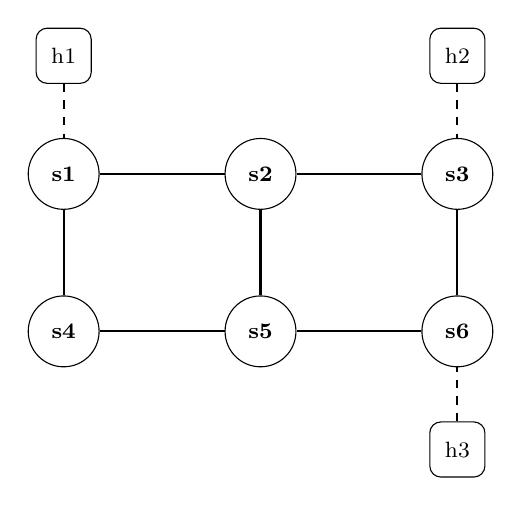
\begin{tikzpicture}[
    sw/.style={draw, circle, minimum size=0.9cm, font=\footnotesize\bfseries},
    host/.style={draw, rectangle, rounded corners, minimum size=0.7cm, font=\footnotesize},
    link/.style={thick},
    node distance=2.5cm
]
% Switches
\node[sw] (s1) at (0, 2) {s1};
\node[sw] (s2) at (2.5, 2) {s2};
\node[sw] (s3) at (5, 2) {s3};
\node[sw] (s4) at (0, 0) {s4};
\node[sw] (s5) at (2.5, 0) {s5};
\node[sw] (s6) at (5, 0) {s6};

% Hosts
\node[host] (h1) at (0, 3.5) {h1};
\node[host] (h2) at (5, 3.5) {h2};
\node[host] (h3) at (5, -1.5) {h3};

% Switch links
\draw[link] (s1) -- (s2);
\draw[link] (s2) -- (s3);
\draw[link] (s4) -- (s5);
\draw[link] (s5) -- (s6);
\draw[link] (s1) -- (s4);
\draw[link] (s2) -- (s5);
\draw[link] (s3) -- (s6);

% Host links
\draw[link, dashed] (h1) -- (s1);
\draw[link, dashed] (h2) -- (s3);
\draw[link, dashed] (h3) -- (s6);
\end{tikzpicture}
\caption{Grid Topology (2$\times$3) --- 6 switches, 3 hosts, multiple equal-cost paths}
\end{figure}

\paragraph{Mesh Topology (Ring + Diagonal):}

A four-switch topology with full mesh connectivity (ring plus diagonal links). Every switch pair is directly connected, providing maximum path redundancy and testing the controller's ability to select the optimal single-hop path.

\begin{figure}[H]
\centering
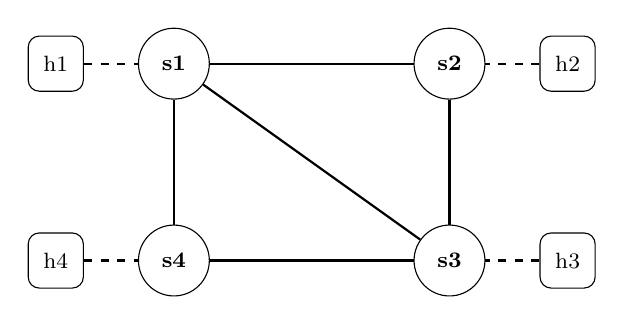
\begin{tikzpicture}[
    sw/.style={draw, circle, minimum size=0.9cm, font=\footnotesize\bfseries},
    host/.style={draw, rectangle, rounded corners, minimum size=0.7cm, font=\footnotesize},
    link/.style={thick},
]
% Switches
\node[sw] (s1) at (0, 2.5) {s1};
\node[sw] (s2) at (3.5, 2.5) {s2};
\node[sw] (s3) at (3.5, 0) {s3};
\node[sw] (s4) at (0, 0) {s4};

% Hosts
\node[host] (h1) at (-1.5, 2.5) {h1};
\node[host] (h2) at (5, 2.5) {h2};
\node[host] (h3) at (5, 0) {h3};
\node[host] (h4) at (-1.5, 0) {h4};

% Switch links (full mesh)
\draw[link] (s1) -- (s2);
\draw[link] (s2) -- (s3);
\draw[link] (s3) -- (s4);
\draw[link] (s4) -- (s1);
\draw[link] (s1) -- (s3);  % diagonal

% Host links
\draw[link, dashed] (h1) -- (s1);
\draw[link, dashed] (h2) -- (s2);
\draw[link, dashed] (h3) -- (s3);
\draw[link, dashed] (h4) -- (s4);
\end{tikzpicture}
\caption{Mesh Topology --- 4 switches fully connected, 4 hosts}
\end{figure}

\paragraph{Triangle Topology:}

A minimal redundant topology with three switches forming a triangle. Tests basic shortest-path selection and failover with the simplest possible redundant structure.

\begin{figure}[H]
\centering
\begin{tikzpicture}[
    sw/.style={draw, circle, minimum size=0.9cm, font=\footnotesize\bfseries},
    host/.style={draw, rectangle, rounded corners, minimum size=0.7cm, font=\footnotesize},
    link/.style={thick},
]
\node[sw] (s1) at (2, 3) {s1};
\node[sw] (s2) at (0, 0) {s2};
\node[sw] (s3) at (4, 0) {s3};

\node[host] (h1) at (2, 4.5) {h1};
\node[host] (h2) at (-1.5, 0) {h2};
\node[host] (h3) at (5.5, 0) {h3};

\draw[link] (s1) -- (s2);
\draw[link] (s2) -- (s3);
\draw[link] (s1) -- (s3);

\draw[link, dashed] (h1) -- (s1);
\draw[link, dashed] (h2) -- (s2);
\draw[link, dashed] (h3) -- (s3);
\end{tikzpicture}
\caption{Triangle Topology --- 3 switches, 3 hosts, minimal redundancy}
\end{figure}

\paragraph{Diamond Topology:}

A four-switch diamond where traffic between h1 and h2 must traverse two intermediate switches. Tests correct multi-hop path computation and ensures the controller selects one of the two equal-cost paths consistently.

\begin{figure}[H]
\centering
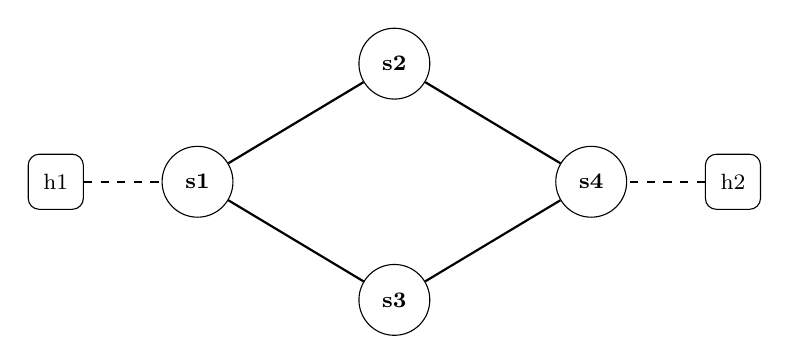
\begin{tikzpicture}[
    sw/.style={draw, circle, minimum size=0.9cm, font=\footnotesize\bfseries},
    host/.style={draw, rectangle, rounded corners, minimum size=0.7cm, font=\footnotesize},
    link/.style={thick},
]
\node[sw] (s1) at (0, 1.5) {s1};
\node[sw] (s2) at (2.5, 3) {s2};
\node[sw] (s3) at (2.5, 0) {s3};
\node[sw] (s4) at (5, 1.5) {s4};

\node[host] (h1) at (-1.8, 1.5) {h1};
\node[host] (h2) at (6.8, 1.5) {h2};

\draw[link] (s1) -- (s2);
\draw[link] (s1) -- (s3);
\draw[link] (s2) -- (s4);
\draw[link] (s3) -- (s4);

\draw[link, dashed] (h1) -- (s1);
\draw[link, dashed] (h2) -- (s4);
\end{tikzpicture}
\caption{Diamond Topology --- 4 switches, 2 hosts, two equal-cost paths}
\end{figure}

\paragraph{Line Topology:}

A simple linear chain of four switches. Tests the controller's handling of a topology with no redundancy, where a single link failure partitions the network.

\begin{figure}[H]
\centering
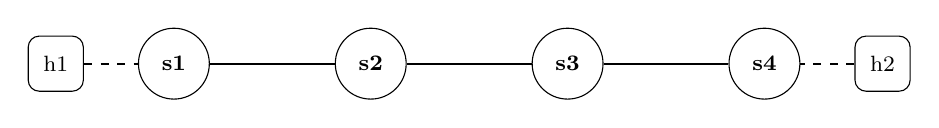
\begin{tikzpicture}[
    sw/.style={draw, circle, minimum size=0.9cm, font=\footnotesize\bfseries},
    host/.style={draw, rectangle, rounded corners, minimum size=0.7cm, font=\footnotesize},
    link/.style={thick},
]
\node[host] (h1) at (-1.5, 0) {h1};
\node[sw] (s1) at (0, 0) {s1};
\node[sw] (s2) at (2.5, 0) {s2};
\node[sw] (s3) at (5, 0) {s3};
\node[sw] (s4) at (7.5, 0) {s4};
\node[host] (h2) at (9, 0) {h2};

\draw[link] (s1) -- (s2);
\draw[link] (s2) -- (s3);
\draw[link] (s3) -- (s4);
\draw[link, dashed] (h1) -- (s1);
\draw[link, dashed] (h2) -- (s4);
\end{tikzpicture}
\caption{Line Topology --- 4 switches in a chain, 2 hosts, no redundancy}
\end{figure}

\paragraph{Heavy Mesh Topology:}

A densely connected 2$\times$3 grid of six switches with additional diagonal cross-links, totalling eleven switch-to-switch edges. Eight hosts are distributed across the network. This topology tests the controller's ability to compute shortest paths through a highly redundant mesh and to reroute traffic when single, double, or even triple link failures occur. Because each switch has at least three switch-to-switch connections, the network can tolerate multiple simultaneous failures before any host becomes isolated.

\begin{figure}[H]
\centering
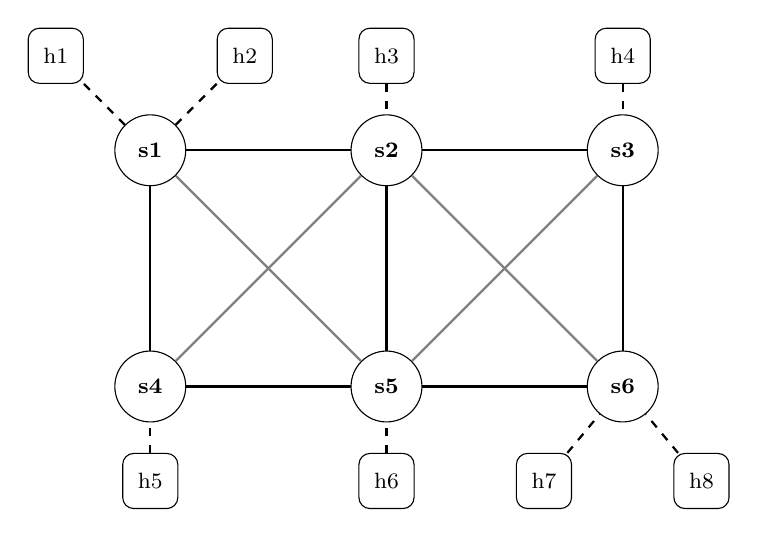
\begin{tikzpicture}[
    sw/.style={draw, circle, minimum size=0.9cm, font=\footnotesize\bfseries},
    host/.style={draw, rectangle, rounded corners, minimum size=0.7cm, font=\footnotesize},
    link/.style={thick},
    cross/.style={thick, gray},
]
% Switches (2x3 grid)
\node[sw] (s1) at (0, 0) {s1};
\node[sw] (s2) at (3, 0) {s2};
\node[sw] (s3) at (6, 0) {s3};
\node[sw] (s4) at (0, -3) {s4};
\node[sw] (s5) at (3, -3) {s5};
\node[sw] (s6) at (6, -3) {s6};

% Hosts
\node[host] (h1) at (-1.2, 1.2) {h1};
\node[host] (h2) at (1.2, 1.2) {h2};
\node[host] (h3) at (3, 1.2) {h3};
\node[host] (h4) at (6, 1.2) {h4};
\node[host] (h5) at (0, -4.2) {h5};
\node[host] (h6) at (3, -4.2) {h6};
\node[host] (h7) at (5.0, -4.2) {h7};
\node[host] (h8) at (7.0, -4.2) {h8};

% Host-to-switch links (dashed)
\draw[link, dashed] (h1) -- (s1);
\draw[link, dashed] (h2) -- (s1);
\draw[link, dashed] (h3) -- (s2);
\draw[link, dashed] (h4) -- (s3);
\draw[link, dashed] (h5) -- (s4);
\draw[link, dashed] (h6) -- (s5);
\draw[link, dashed] (h7) -- (s6);
\draw[link, dashed] (h8) -- (s6);

% Horizontal links
\draw[link] (s1) -- (s2);
\draw[link] (s2) -- (s3);
\draw[link] (s4) -- (s5);
\draw[link] (s5) -- (s6);

% Vertical links
\draw[link] (s1) -- (s4);
\draw[link] (s2) -- (s5);
\draw[link] (s3) -- (s6);

% Cross-links (diagonals)
\draw[cross] (s1) -- (s5);
\draw[cross] (s2) -- (s4);
\draw[cross] (s2) -- (s6);
\draw[cross] (s3) -- (s5);

\end{tikzpicture}
\caption{Heavy Mesh Topology --- 6 switches in a 2$\times$3 grid with cross-links, 8 hosts, 11 switch-to-switch links}
\end{figure}

% \subsubsection{Test Cases}

% \begin{table}[H]
% \centering
% \begin{tabular}{@{}p{4.5cm}p{5cm}p{3.5cm}@{}}
% \toprule
% \textbf{Test Case} & \textbf{Verification} & \textbf{Topology} \\
% \midrule
% \texttt{test\_pingall} & Full mesh connectivity with 0\% loss & All topologies \\
% \texttt{test\_shortest\_path} & Path length matches expected hop count & Grid, Mesh, Diamond \\
% \texttt{test\_link\_failure} & Connectivity maintained after link down & Mesh, Triangle, Grid \\
% \texttt{test\_link\_recovery} & Optimal path restored after link up & Mesh, Triangle \\
% \texttt{test\_no\_redundancy\_failure} & Correct behaviour when no alternate path exists & Line \\
% \bottomrule
% \end{tabular}
% \caption{Switching Test Cases}
% \end{table}

\subsubsection{Results}

\begin{center}
\fbox{\textbf{\large All switching tests: PASSED} \checkmark}
\end{center}

% ----------------------------------------
\subsection{DHCP Tests}

\subsubsection{What It Verifies}

The DHCP test suite validates that the controller's built-in DHCP server correctly allocates IP addresses to hosts, handling the complete DHCP lifecycle:

\begin{itemize}[leftmargin=1.5cm]
    \item \textbf{Basic DHCP (\texttt{test\_network.py}):} Hosts broadcast a DHCP DISCOVER message and receive a valid OFFER with an IP from the configured pool. Hosts confirm the offered address via REQUEST and receive an ACK with correct lease parameters. Multiple hosts receive distinct IP addresses with no conflicts, and all allocated addresses fall within the pool range.
    \item \textbf{DHCP RELEASE (\texttt{test\_network.py}):} (Bonus) A host releases its DHCP lease; the IP is returned to the pool and can be re-issued to another host. The test uses pool exhaustion to prove that a released IP is truly reclaimed.
    \item \textbf{Duplicate IP Rejection (\texttt{test\_network.py}):} (Bonus) A host attempts to steal an IP that is already bound to another host. The server responds with DHCPNAK and either assigns a different IP or leaves the client without a valid address.
    \item \textbf{Overflow (\texttt{test\_network\_overflow.py}):} (Bonus) Deploys more hosts than available pool addresses and verifies that the server correctly handles pool exhaustion --- the last host(s) fail to obtain an IP.
    \item \textbf{Lease Expiry (\texttt{test\_lease\_expiry.py}):} (Bonus) Validates that expired leases are automatically reclaimed. Requires manually setting a short \texttt{Config.lease\_time} (e.g., 5 seconds) and a 2-IP pool (\texttt{end\_ip="192.168.1.3"}). Uses 3 hosts: h1 and h2 exhaust the pool, h1's dhclient is killed and IP stripped, then a fresh third host (h3) fails to obtain an IP before the timeout but succeeds afterward --- proving the lease expired and was reclaimed.
\end{itemize}

\subsubsection{Test Topology}

The interactive test uses a single-switch topology with 3 hosts (to enable pool exhaustion in the release test when the pool is small).

\begin{figure}[H]
\centering
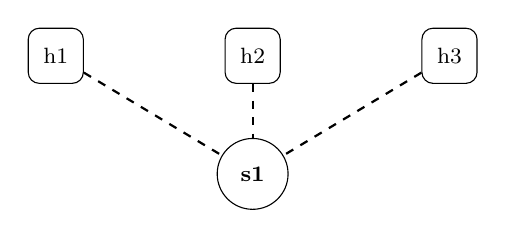
\begin{tikzpicture}[
    sw/.style={draw, circle, minimum size=0.9cm, font=\footnotesize\bfseries},
    host/.style={draw, rectangle, rounded corners, minimum size=0.7cm, font=\footnotesize},
    link/.style={thick},
]
\node[sw] (s1) at (2.5, 0) {s1};
\node[host] (h1) at (0, 1.5) {h1};
\node[host] (h2) at (2.5, 1.5) {h2};
\node[host] (h3) at (5, 1.5) {h3};

\draw[link, dashed] (h1) -- (s1);
\draw[link, dashed] (h2) -- (s1);
\draw[link, dashed] (h3) -- (s1);
\end{tikzpicture}
\caption{DHCP Test Topology --- single switch, up to 3 hosts (h3 used for pool-exhaustion release tests)}
\end{figure}

\subsubsection{Test Cases}

\begin{table}[H]
\centering
\begin{tabular}{@{}p{5cm}p{4.5cm}p{4cm}@{}}
\toprule
\textbf{Test Case} & \textbf{Verification} & \textbf{Source File} \\
\midrule
\texttt{test\_basic\_dhcp} & Three hosts each get a valid, unique pool IP & \texttt{test\_network.py} \\
\texttt{test\_dhcp\_release} & Released IP is returned to pool and re-issued & \texttt{test\_network.py} \\
\texttt{test\_duplicate\_ip} & Server sends NAK for stolen IP; host gets different IP or no IP & \texttt{test\_network.py} \\
\texttt{test\_overflow} & More hosts than pool IPs; excess hosts fail to get IP & \texttt{test\_network\_overflow.py} \\
\texttt{test\_lease\_expiry} & Expired lease reclaimed after timeout; fresh host gets same IP & \texttt{test\_lease\_expiry.py} \\
\bottomrule
\end{tabular}
\caption{DHCP Test Cases}
\end{table}

\subsubsection{Results}

\begin{center}
\fbox{\textbf{\large All DHCP tests: PASSED} \checkmark}
\end{center}

% ----------------------------------------
\subsection{Firewall Tests}

\subsubsection{What It Verifies}

The firewall test suite validates that deny rules loaded from \texttt{firewall\_rules.json} are correctly translated into high-priority drop flows (priority 60000) and enforced at the data plane across multiple topologies and rule configurations. The suite covers three test files:

\begin{itemize}[leftmargin=1.5cm]
    \item \textbf{CIDR Subnet Mask Testing (\texttt{test\_network\_firewall\_mask.py}):} A test that verifies CIDR subnet mask support in firewall rules. It validates that /30 masks correctly include only hosts within the subnet range (e.g., 192.168.117.0/30 covers .0--.3) while excluding hosts outside, and similarly for /31 masks. Six targeted tests verify both ICMP and TCP port filtering with exact subnet boundaries.
    \item \textbf{HeavyMesh Complexity Test (\texttt{test\_network\_firewall\_complexity.py}):} A test that combines firewall enforcement with shortest-path switching on a HeavyMesh topology (6 switches, 8 hosts, 11 switch-to-switch links). Two modes are supported: \textbf{connect} (empty ruleset --- all $C(8,2)=28$ host pairs must be reachable, verifying the firewall does not interfere when inactive) and \textbf{disconnect} (4 bidirectional deny rules blocking h1$\leftrightarrow$h3 and h5$\leftrightarrow$h8 ICMP). In disconnect mode, even though multiple redundant paths exist between the blocked hosts' switches, the firewall drop flows must take precedence at priority 60000. A batch parallel ping mechanism is used to efficiently test all 56 directed ping pairs simultaneously.
    \item \textbf{Basic Firewall Test (\texttt{test\_network.py}):} A test on the basic single-switch topology that starts HTTP servers on h2 (ports 80 and 8080), then runs ICMP ping and TCP curl tests. It also performs a \texttt{pingAll} to verify the firewall filtering effect.
\end{itemize}

\subsubsection{Test Topologies}

\paragraph{Simple Topology (used by \texttt{test\_network.py}, \texttt{test\_network\_firewall\_mask.py})}

\begin{figure}[H]
\centering
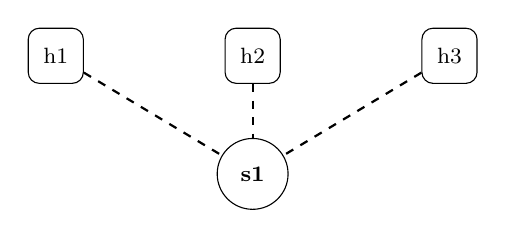
\begin{tikzpicture}[
    sw/.style={draw, circle, minimum size=0.9cm, font=\footnotesize\bfseries},
    host/.style={draw, rectangle, rounded corners, minimum size=0.7cm, font=\footnotesize},
    link/.style={thick},
]
\node[sw] (s1) at (2.5, 0) {s1};
\node[host] (h1) at (0, 1.5) {h1};
\node[host] (h2) at (2.5, 1.5) {h2};
\node[host] (h3) at (5, 1.5) {h3};

\draw[link, dashed] (h1) -- (s1);
\draw[link, dashed] (h2) -- (s1);
\draw[link, dashed] (h3) -- (s1);
\end{tikzpicture}
\caption{Firewall Simple Test Topology --- single switch, 3 hosts}
\end{figure}

\paragraph{HeavyMesh Topology (used by \texttt{test\_network\_firewall\_complexity.py})}

\begin{figure}[H]
\centering
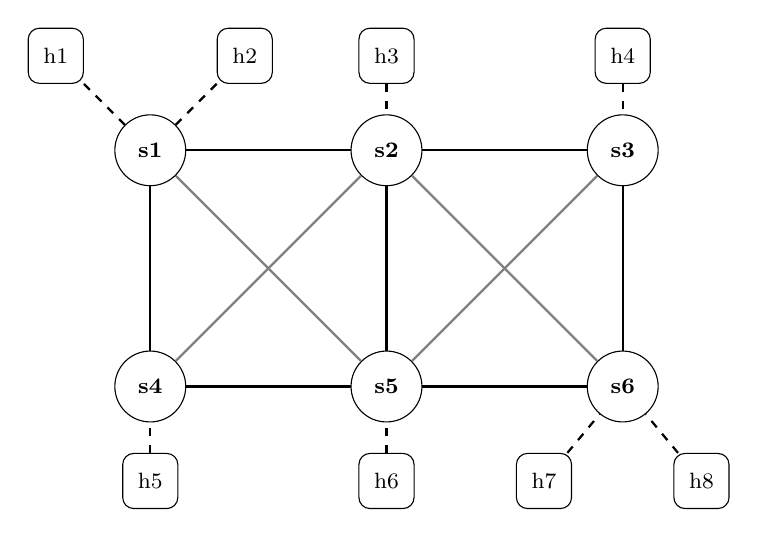
\begin{tikzpicture}[
    sw/.style={draw, circle, minimum size=0.9cm, font=\footnotesize\bfseries},
    host/.style={draw, rectangle, rounded corners, minimum size=0.7cm, font=\footnotesize},
    link/.style={thick},
    cross/.style={thick, gray},
]
% Switches (2x3 grid)
\node[sw] (s1) at (0, 0) {s1};
\node[sw] (s2) at (3, 0) {s2};
\node[sw] (s3) at (6, 0) {s3};
\node[sw] (s4) at (0, -3) {s4};
\node[sw] (s5) at (3, -3) {s5};
\node[sw] (s6) at (6, -3) {s6};

% Hosts
\node[host] (h1) at (-1.2, 1.2) {h1};
\node[host] (h2) at (1.2, 1.2) {h2};
\node[host] (h3) at (3, 1.2) {h3};
\node[host] (h4) at (6, 1.2) {h4};
\node[host] (h5) at (0, -4.2) {h5};
\node[host] (h6) at (3, -4.2) {h6};
\node[host] (h7) at (5.0, -4.2) {h7};
\node[host] (h8) at (7.0, -4.2) {h8};

% Host-to-switch links (dashed)
\draw[link, dashed] (h1) -- (s1);
\draw[link, dashed] (h2) -- (s1);
\draw[link, dashed] (h3) -- (s2);
\draw[link, dashed] (h4) -- (s3);
\draw[link, dashed] (h5) -- (s4);
\draw[link, dashed] (h6) -- (s5);
\draw[link, dashed] (h7) -- (s6);
\draw[link, dashed] (h8) -- (s6);

% Horizontal links
\draw[link] (s1) -- (s2);
\draw[link] (s2) -- (s3);
\draw[link] (s4) -- (s5);
\draw[link] (s5) -- (s6);

% Vertical links
\draw[link] (s1) -- (s4);
\draw[link] (s2) -- (s5);
\draw[link] (s3) -- (s6);

% Cross-links (diagonals)
\draw[cross] (s1) -- (s5);
\draw[cross] (s2) -- (s4);
\draw[cross] (s2) -- (s6);
\draw[cross] (s3) -- (s5);
\end{tikzpicture}
\caption{Firewall HeavyMesh Test Topology --- 6 switches, 8 hosts, 11 switch-to-switch links}
\end{figure}

\subsubsection{Test Cases}

\begin{table}[H]
\centering
\begin{tabular}{@{}p{5cm}p{4.5cm}p{4cm}@{}}
\toprule
\textbf{Test Case} & \textbf{Verification} & \textbf{Source File} \\
\midrule
\texttt{test\_cidr30\_match} & /30 mask: h1 (.2) in 192.168.117.0/30, blocked & \texttt{test\_network\_firewall\_mask.py} \\
\texttt{test\_cidr30\_nomatch} & /30 mask: h3 (.4) not in 192.168.117.0/30, allowed & \texttt{test\_network\_firewall\_mask.py} \\
\texttt{test\_cidr31\_match} & /31 mask: h3 (.4) in 192.168.117.4/31, blocked & \texttt{test\_network\_firewall\_mask.py} \\
\texttt{test\_cidr31\_nomatch} & /31 mask: h1 (.2) not in 192.168.117.4/31, allowed & \texttt{test\_network\_firewall\_mask.py} \\
\texttt{test\_heavymesh\_connect} & All 28 host pairs reachable (empty ruleset) & \texttt{test\_network\_firewall\_complexity.py} \\
\texttt{test\_heavymesh\_disconnect} & h1$\leftrightarrow$h3, h5$\leftrightarrow$h8 blocked; all other 24 pairs reachable & \texttt{test\_network\_firewall\_complexity.py} \\
\bottomrule
\end{tabular}
\caption{Firewall Test Cases}
\end{table}

\subsubsection{Results}

\begin{center}
\fbox{\textbf{\large All firewall tests: PASSED} \checkmark}
\end{center}

\textbf{TODO: Paste experimental output here.}

% ----------------------------------------
\subsection{DNS Tests}

\subsubsection{What It Verifies}

The DNS test suite validates the in-controller DNS resolution service across two topologies and two test files. Hosts obtain IP addresses via the built-in DHCP server, send gratuitous ARP to register with the controller, and then perform DNS queries using \texttt{dig} against the DNS server at 192.168.1.1:

\begin{itemize}[leftmargin=1.5cm]
    \item \textbf{Basic DNS Test (\texttt{test\_network\_dns.py}):} A test on the simple single-switch topology. After DHCP and ARP registration, it verifies: A-record resolution of \texttt{h2.local} and \texttt{h1.local}, NXDOMAIN for \texttt{nonexistent.local}, and PTR reverse lookups for both hosts' IPs.
    \item \textbf{Complex Multi-Switch DNS Test (\texttt{test\_network\_dns\_complex.py}):} A test on a 4-switch mesh topology with 6 hosts distributed across switches (h1 on s1, h2 on s2, h3/h5 on s3, h4/h6 on s4). Five test categories are covered: (1) same-switch A-record resolution (h3 $\\leftrightarrow$ h5 on s3; h4 $\\leftrightarrow$ h6 on s4); (2) 1-hop A-record resolution (h1 $\\leftrightarrow$ h3 via direct s1--s3 link); (3) 2-hop A-record resolution (h2 $\\leftrightarrow$ h5, h1 $\\leftrightarrow$ h6); (4) full cross-resolution --- every host resolves every other host's \texttt{*.local} name (30 directed queries); (5) NXDOMAIN for various non-existent hostnames. This test validates that DNS resolution works correctly regardless of the number of switch hops between the querying host and the DNS server.
\end{itemize}

\subsubsection{Test Topologies}

\paragraph{Simple Topology (used by \texttt{test\_network\_dns.py})}

\begin{figure}[H]
\centering
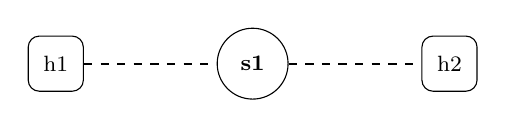
\begin{tikzpicture}[
    sw/.style={draw, circle, minimum size=0.9cm, font=\footnotesize\bfseries},
    host/.style={draw, rectangle, rounded corners, minimum size=0.7cm, font=\footnotesize},
    link/.style={thick},
]
\node[host] (h1) at (0, 0) {h1};
\node[sw] (s1) at (2.5, 0) {s1};
\node[host] (h2) at (5, 0) {h2};

\draw[link, dashed] (h1) -- (s1);
\draw[link, dashed] (s1) -- (h2);
\end{tikzpicture}
\caption{DNS Simple Test Topology --- single switch, 2 hosts}
\end{figure}

\paragraph{Complex Mesh Topology (used by \texttt{test\_network\_dns\_complex.py})}

\begin{figure}[H]
\centering
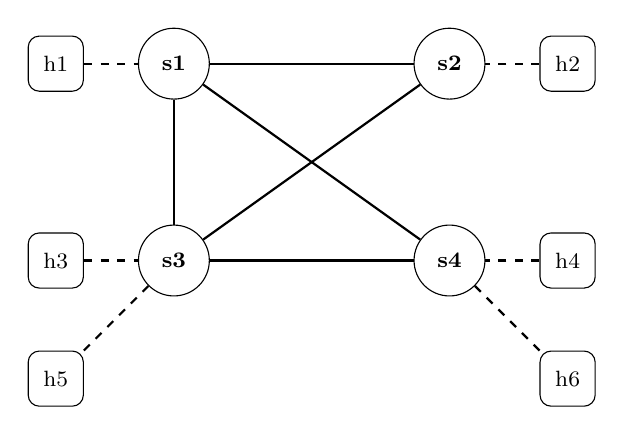
\begin{tikzpicture}[
    sw/.style={draw, circle, minimum size=0.9cm, font=\footnotesize\bfseries},
    host/.style={draw, rectangle, rounded corners, minimum size=0.7cm, font=\footnotesize},
    link/.style={thick},
]
% Switches
\node[sw] (s1) at (0, 2.5) {s1};
\node[sw] (s2) at (3.5, 2.5) {s2};
\node[sw] (s3) at (0, 0) {s3};
\node[sw] (s4) at (3.5, 0) {s4};

% Hosts
\node[host] (h1) at (-1.5, 2.5) {h1};
\node[host] (h2) at (5, 2.5) {h2};
\node[host] (h3) at (-1.5, 0) {h3};
\node[host] (h4) at (5, 0) {h4};
\node[host] (h5) at (-1.5, -1.5) {h5};
\node[host] (h6) at (5, -1.5) {h6};

% Switch-to-switch links (mesh)
\draw[link] (s1) -- (s2);
\draw[link] (s1) -- (s3);
\draw[link] (s1) -- (s4);
\draw[link] (s2) -- (s3);
\draw[link] (s3) -- (s4);

% Host-to-switch links (dashed)
\draw[link, dashed] (h1) -- (s1);
\draw[link, dashed] (h2) -- (s2);
\draw[link, dashed] (h3) -- (s3);
\draw[link, dashed] (h4) -- (s4);
\draw[link, dashed] (h5) -- (s3);
\draw[link, dashed] (h6) -- (s4);
\end{tikzpicture}
\caption{DNS Complex Mesh Test Topology --- 4 switches, 6 hosts, 5 switch-to-switch links}
\end{figure}

\subsubsection{Test Cases}

\begin{table}[H]
\centering
\begin{tabular}{@{}p{5cm}p{4.5cm}p{4cm}@{}}
\toprule
\textbf{Test Case} & \textbf{Verification} & \textbf{Source File} \\
\midrule
\texttt{test\_dns\_same\_switch} & Hosts on same switch resolve each other (h3$\\leftrightarrow$h5, h4$\\leftrightarrow$h6) & \texttt{test\_network\_dns\_complex.py} \\
\texttt{test\_dns\_one\_hop} & Hosts 1 switch hop apart resolve correctly (h1$\\leftrightarrow$h3, h2$\\leftrightarrow$h4) & \texttt{test\_network\_dns\_complex.py} \\
\texttt{test\_dns\_two\_hops} & Hosts 2 switch hops apart resolve correctly (h2$\\leftrightarrow$h5, h1$\\leftrightarrow$h6) & \texttt{test\_network\_dns\_complex.py} \\
\texttt{test\_dns\_full\_cross} & Every host resolves every other host (30 directed queries) & \texttt{test\_network\_dns\_complex.py} \\
\texttt{test\_dns\_nxdomain\_various} & Multiple non-existent hostnames all return NXDOMAIN & \texttt{test\_network\_dns\_complex.py} \\
\bottomrule
\end{tabular}
\caption{DNS Test Cases}
\end{table}

\subsubsection{Results}

\begin{center}
\fbox{\textbf{\large All DNS tests: PASSED} \checkmark}
\end{center}

\textbf{TODO: Paste experimental output here.}

% ----------------------------------------
\subsection{NAT Tests}

\subsubsection{What It Verifies}

The NAT test suite validates correct address translation (SNAT/DNAT) between the internal subnet (10.0.1.0/24) and external subnet (10.0.2.0/24) across three test files covering basic connectivity, multi-host scenarios, and protocol-level correctness:

\begin{itemize}[leftmargin=1.5cm]
    \item \textbf{Basic NAT Test (\texttt{test\_network\_nat.py}):} A test on the basic two-switch topology. It performs three tests: (1) h1 $\\rightarrow$ h2 ping (SNAT outbound); (2) h2 $\\rightarrow$ h1 ping (DNAT inbound); (3) SNAT source verification via a TCP server on h2 that logs the connecting client IP.
    \item \textbf{Multi-Host NAT Test (\texttt{test\_network\_nat\_multi.py}):} A test with 4 internal hosts (h1--h4: 10.0.1.2--10.0.1.5) and 3 external hosts (h5--h7: 10.0.2.2--10.0.2.4) on a two-switch topology. Four test categories: (1) all 12 internal$\\rightarrow$external ping pairs; (2) all 3 external hosts ping NAT_IP (10.0.2.100) via DNAT; (3) SNAT verification --- all 4 internal hosts connect via TCP to a single external observer (h5), which must see all connections sourced from the NAT external IP (10.0.2.100) but with \\textbf{different translated ports}, proving port uniqueness across concurrent connections; (4) internal hosts can also reach other external hosts beyond the observer.
    \item \textbf{Protocol Coverage Test (\texttt{test\_network\_nat\_proto.py}):} A test on the basic two-switch topology that exercises all three transport protocols through NAT. \\textbf{ICMP:} single-flow ping (h1$\\rightarrow$h2 and reverse), plus two concurrent pings from h1 to h2 launched simultaneously to verify ICMP identifier-based connection tracking can distinguish separate flows. \\textbf{UDP:} a UDP echo server on h2 (port 22348) receives a datagram from h1 and echoes it back with an \texttt{ECHO:} prefix, validating connectionless UDP translation. \\textbf{TCP:} a TCP echo server on h2 (port 22349) accepts a connection from h1, receives data, and sends back \texttt{ECHO:} prefixed response, validating connection-oriented TCP stream translation and bidirectional checksum correctness.
\end{itemize}

\subsubsection{Test Topologies}

\paragraph{Basic Topology (used by \texttt{test\_network\_nat.py}, \texttt{test\_network\_nat\_proto.py})}

\begin{figure}[H]
\centering
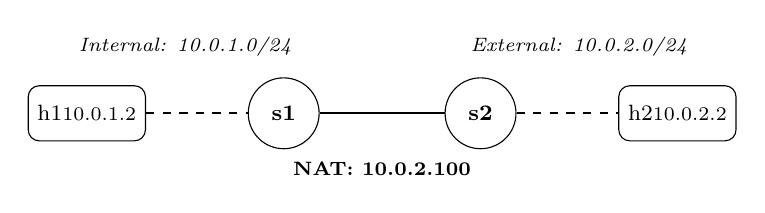
\begin{tikzpicture}[
    sw/.style={draw, circle, minimum size=0.9cm, font=\footnotesize\bfseries},
    host/.style={draw, rectangle, rounded corners, minimum size=0.7cm, font=\footnotesize},
    link/.style={thick},
]
\node[host] (h1) at (0, 0) {h1\\{\scriptsize 10.0.1.2}};
\node[sw] (s1) at (2.5, 0) {s1};
\node[sw] (s2) at (5, 0) {s2};
\node[host] (h2) at (7.5, 0) {h2\\{\scriptsize 10.0.2.2}};

\draw[link, dashed] (h1) -- (s1);
\draw[link] (s1) -- (s2);
\draw[link, dashed] (s2) -- (h2);

% Subnet labels
\node[above, font=\scriptsize\itshape] at (1.25, 0.6) {Internal: 10.0.1.0/24};
\node[above, font=\scriptsize\itshape] at (6.25, 0.6) {External: 10.0.2.0/24};

% NAT label
\node[below, font=\scriptsize\bfseries] at (3.75, -0.5) {NAT: 10.0.2.100};
\end{tikzpicture}
\caption{NAT Basic Test Topology --- 2 switches, 2 hosts in different subnets}
\end{figure}

\paragraph{Multi-Host Topology (used by \texttt{test\_network\_nat\_multi.py})}

\begin{figure}[H]
\centering
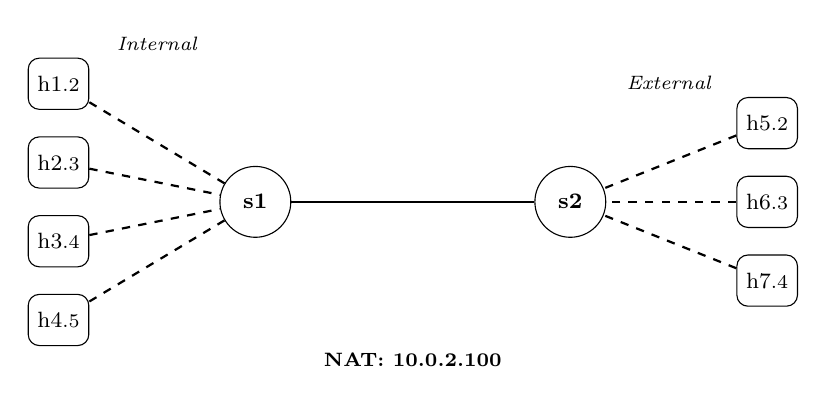
\begin{tikzpicture}[
    sw/.style={draw, circle, minimum size=0.9cm, font=\footnotesize\bfseries},
    host/.style={draw, rectangle, rounded corners, minimum size=0.65cm, font=\footnotesize},
    link/.style={thick},
]
% Switches
\node[sw] (s1) at (2.5, 0) {s1};
\node[sw] (s2) at (6.5, 0) {s2};

% Internal hosts (left side)
\node[host] (h1) at (0, 1.5) {h1\\{\scriptsize .2}};
\node[host] (h2) at (0, 0.5) {h2\\{\scriptsize .3}};
\node[host] (h3) at (0, -0.5) {h3\\{\scriptsize .4}};
\node[host] (h4) at (0, -1.5) {h4\\{\scriptsize .5}};

% External hosts (right side)
\node[host] (h5) at (9, 1.0) {h5\\{\scriptsize .2}};
\node[host] (h6) at (9, 0) {h6\\{\scriptsize .3}};
\node[host] (h7) at (9, -1.0) {h7\\{\scriptsize .4}};

% Host-to-switch links
\draw[link, dashed] (h1) -- (s1);
\draw[link, dashed] (h2) -- (s1);
\draw[link, dashed] (h3) -- (s1);
\draw[link, dashed] (h4) -- (s1);
\draw[link, dashed] (h5) -- (s2);
\draw[link, dashed] (h6) -- (s2);
\draw[link, dashed] (h7) -- (s2);

% Switch-to-switch link
\draw[link] (s1) -- (s2);

% Labels
\node[above, font=\scriptsize\itshape] at (1.25, 1.8) {Internal};
\node[above, font=\scriptsize\itshape] at (7.75, 1.3) {External};
\node[below, font=\scriptsize\bfseries] at (4.5, -1.8) {NAT: 10.0.2.100};
\end{tikzpicture}
\caption{NAT Multi-Host Test Topology --- 4 internal hosts, 3 external hosts, 2 switches}
\end{figure}

\subsubsection{Test Cases}

\begin{table}[H]
\centering
\begin{tabular}{@{}p{5cm}p{4.5cm}p{4cm}@{}}
\toprule
\textbf{Test Case} & \textbf{Verification} & \textbf{Source File} \\
\midrule
\texttt{test\_nat\_multi\_ping\_out} & All 12 internal$\\rightarrow$external ping pairs succeed & \texttt{test\_network\_nat\_multi.py} \\
\texttt{test\_nat\_multi\_ping\_in} & All 3 external hosts ping NAT_IP (10.0.2.100) via DNAT & \texttt{test\_network\_nat\_multi.py} \\
\texttt{test\_nat\_port\_uniqueness} & 4 internal hosts get 4 distinct translated ports on NAT IP & \texttt{test\_network\_nat\_multi.py} \\
\texttt{test\_nat\_icmp\_concurrent} & Two simultaneous pings from h1 to h2 both succeed (separate ICMP flows) & \texttt{test\_network\_nat\_proto.py} \\
\texttt{test\_nat\_udp\_echo} & UDP echo server on h2:22348 echoes back \texttt{ECHO:HELLO} from h1 & \texttt{test\_network\_nat\_proto.py} \\
\texttt{test\_nat\_tcp\_echo} & TCP echo server on h2:22349 echoes back \texttt{ECHO:HELLO} from h1 & \texttt{test\_network\_nat\_proto.py} \\
\bottomrule
\end{tabular}
\caption{NAT Test Cases}
\end{table}

\subsubsection{Results}

\begin{center}
\fbox{\textbf{\large All NAT tests: PASSED} \checkmark}
\end{center}

\textbf{TODO: Paste experimental output here.}

% ============================================================
\end{document}